\documentclass[aspectratio=169]{beamer}

% setup basic metainfo
\title{Reducing Optimism Bias in Incomplete Cooperative Games}
\author[1]{Filip \'{U}radn\'{i}k\textsuperscript{1} \and David Sychrovský\textsuperscript{1} \and Jakub Černý\textsuperscript{2}\and Martin Černý\textsuperscript{1}}

\institute{
    \textsuperscript{1}Charles University, Prague\hfill \\
    \textsuperscript{2}Columbia University, NY, USA\hfill \\

\vspace{1em}
{\tiny\color{gray}
\texttt{uradnik@kam.mff.cuni.cz}
\hspace{1em}\textbullet\hspace{1em}
\texttt{furadnik.github.io}}
}
\date{October 30, 2025}

\usepackage[utf8]{inputenc}
\usepackage{csquotes}
\usepackage{graphicx, xcolor}
\usepackage{mfirstuc}
%\usepackage[defaultmono]{droidmono}
\usepackage{amsmath,amssymb,amsthm,textcomp,thm-restate}
\usepackage{listings}
\usepackage{parskip}
\usepackage{stmaryrd} % lightning symbol n stuff
\usepackage[noend]{algpseudocode}
\usepackage{tikz}
\usepackage{indentfirst}
\usetikzlibrary{positioning}


% handle fonts encoding.
\usepackage[utf8]{inputenc}
\usepackage[T1]{fontenc}

% hyperlinks
\usepackage[capitalize]{cleveref}
\hypersetup{
	colorlinks=false
}

\numberwithin{equation}{section}
\numberwithin{equation}{subsection}
\renewcommand*{\theequation}{%
	\ifnum\value{subsection}=0 %
		\ifnum\value{section}=0 %
		\else\thesection.\fi\else\thesubsection.\fi\arabic{equation}%
}

% small matrix with parenths
\newenvironment{psmallmatrix} {\left(\begin{smallmatrix}} {\end{smallmatrix}\right)}

\algrenewcommand\algorithmicthen{\textbf{:}}
\algrenewcommand\algorithmicdo{\textbf{:}}
\algrenewcommand\algorithmicelse{\textbf{else :}}
\algdef{SN}[SUBALG]{Indent}{EndIndent}{}{}%
\algdef{SN}[SUBALG]{Procedure}{EndProcedure}[2]{\algofont{#1}({#2}):}{}%

% acronyms
%\usepackage[automake]{glossaries-extra}
%\setabbreviationstyle[acronym]{long-short}
%\newacronym{satnarka}{PŠ}{Princip Šatnářky}
%\makeglossaries

% text spread on page
% \usepackage{geometry}
% \geometry{left=25mm,right=25mm,%
% 	bindingoffset=0mm, top=20mm,bottom=20mm}

\def\theorempre{1.7ex plus 1.2ex minus 0.6ex}
\def\theorempost{1.5ex plus 1.2ex minus 0.6ex}

% % custom theorems
% \newtheoremstyle{Sdefi}{\theorempre}{\theorempost}{\normalfont}{0pt}
% {\scshape}{: }{0pt}{{\thmname{#1 }}{\thmnumber{#2}}{\thmnote{ (#3)}}}
% \newtheoremstyle{Sthm}{\theorempre}{\theorempost}{\normalfont}{0pt}
% {\scshape}{: }{0pt}{{\thmname{#1 }}{\thmnumber{#2}}{\thmnote{ (#3)}}}
% \newtheoremstyle{Sex}{\theorempre}{\theorempost}{\normalfont}{0pt}
% {\scshape}{: }{0pt}{{\thmname{#1 }}{\thmnumber{#2}}{\thmnote{ (#3)}}}

\renewcommand{\qedsymbol}{$\blacksquare$}
\def\qed{{\parfillskip=0pt\allowbreak\hfill\nobreak $\blacksquare$\par}}

% code listing settings
\lstset{
	language=Python,
	%basicstyle=\ttfamily\small,
	%backgroundcolor=\color{lightgray},
	aboveskip={1.0\baselineskip},
	belowskip={1.0\baselineskip},
	columns=fixed,
	xleftmargin=2\parindent,
	extendedchars=true,
	breaklines=true,
	tabsize=4,
	prebreak=\raisebox{0ex}[0ex][0ex]{\ensuremath{\hookleftarrow}},
	showtabs=false,
	showspaces=false,
	showstringspaces=false,
	%keywordstyle=\color{blue},
	%commentstyle=\color{teal},
	%stringstyle=\color{teal},
	numbers=left,
	captionpos=b
}

% misc
\def\restrict#1#2{#1\!\restriction\!#2}
\def\doubleunderline#1{\underline{\underline{#1}}}
\def\rand#1{\text{#1}}
\def\randvec#1{\textbf{#1}}

\def\suchthat{\;\vert\;}
\def\given{;}

\def\pot#1{\fce{\mathcal{P}}{#1}}
\def\potfin#1{\left[ #1 \right]^{<\omega}}
\def\xor{\mathbin{\oplus}}
\def\divides{\mathbin{\backslash}}

% functions with auto parenths
\def\bfce#1#2{#1\!\bigl(#2\bigr)}
\def\fce#1#2{#1\!\left(#2\right)}
\def\fceb#1#2{#1\!\left[ #2 \right]}
\def\fcec#1#2{#1\{#2\}}
\def\fces#1#2{#1\!\left< #2 \right>}

\def\algofont{\textsc}
\def\algref#1{\algofont{\nameref{#1}}}
\def\algorithm#1#2{\fce{\algofont{#1}}{#2}}
\newenvironment{algor}[3]{\begin{minipage}{\textwidth}\begin{algo}[#1]\ \\ \AlgIn #2\\\AlgOut #3 \begin{algorithmic}[1]}{\end{algorithmic}\end{algo}\end{minipage}}

\def\set#1{\left\{#1\right\}}
\def\arr#1{\left[#1\right]}

\DeclareMathOperator{\conv}{conv}
\DeclareMathOperator{\cov}{cov}
\DeclareMathOperator{\var}{var}
\DeclareMathOperator{\fin}{Fin}
\DeclareMathOperator{\poly}{poly}
\DeclareMathOperator{\dlog}{dlog}
\DeclareMathOperator{\dom}{dom}
\DeclareMathOperator{\rng}{rng}
\DeclareMathOperator*{\argmin}{arg\,min}
\DeclareMathOperator*{\argmax}{arg\,max}
\DeclareMathOperator{\id}{id}
\DeclareMathOperator{\sgn}{sgn}
\DeclareMathOperator{\adj}{adj}
\DeclareMathOperator{\Ker}{Ker}
\DeclareMathOperator{\rank}{rank}
\DeclareMathOperator{\trace}{trace}
\DeclareMathOperator*{\mini}{mini}
\DeclareMathOperator*{\maxi}{maxi}
\DeclareMathOperator*{\avg}{avg}

\def\funcs#1#2{^{#1}#2} % množina funkcí z #1 do #2

\def\isomorph{\cong}
\def\dd{\,\text{d}}
\def\compl#1{\overline {#1}}
\def\tuple#1{\left< #1 \right>}

\def\range#1{\left[ #1 \right]}

% vectors
\def\tr{{\!\top\!}}
\def\trans#1{{#1}^{\tr}}
\def\vec{\boldsymbol}
\def\Rmm#1#2{\R^{#1 \times #2}}
\def\Rm#1{\R^{#1}}
\def\ii#1#2{_{#1,#2}}
\def\inv#1{#1^{\inve}}
\def\inve{-1}
\def\I#1{I_{#1}}
\def\zero{\vec{o}}

% probability and random variables
\def\pr#1{\fceb{\Pr}{#1}}
\def\prfa#1#2{\fceb{\Pr_{#1}}{#2}}
\def\prt#1{\fceb{\Pr}{\text{#1}}}
\def\prfat#1#2{\prfa{#1}{\text{#2}}}
\def\vrv{\textbf}
\def\rv{\text}
\DeclareMathOperator*{\E}{\mathbb{E}}

% distributions
\def\Normd{\mathcal{N}}
\def\normd{\fce{\Normd}}
\def\normdf#1#2#3{\normd{#3 \given #1, #2}}
\DeclareMathOperator{\Berd}{Ber}
\def\berd{\fce{\Berd}}
\def\berdf#1#2{\berd{#2 \given #1}}
\DeclareMathOperator{\Poisd}{Pois}
\def\poisd{\fce{\Poisd}}
\def\poisdf#1#2{\poisd{#2 \given #1}}

\def\Rowsp#1{\mathcal{R}\!\left(#1\right)}
\def\Colsp#1{\mathcal{S}\!\left(#1\right)}

\def\norm#1{\left\lVert #1 \right\rVert }
\def\aabsolute#1{\left\lVert #1 \right\rVert }
\def\absolute#1{\left\lvert #1 \right\rvert }
\def\dotpr#1#2{\langle #1 , #2 \rangle}
\def\randin{\in_R}

\def\emod#1{\mathbin{\equiv_{#1}}}
\def\po{\mathbin{\circ}}

\def\disjcup{\mathbin{\dot\cup}}
\def\bigdisjcup{\mathop{\dot\bigcup}}

\def\deltap{\delta^+}
\def\deltam{\delta^-}

\def\deq{\mathbin{:=}}
\def \lHeq{\mathbin{\stackrel{l'H}{=}}}
\def\concat{\cdot}

\def\R{\mathbb{R}}
\def\Q{\mathbb{Q}}
\def\N{\mathbb{N}}
\def\C{\mathbb{C}}
\def\Z{\mathbb{Z}}
\def\K{\mathbb{K}}
\def\P{\mathbb{P}}
\def\V{\mathbb{V}}
\def\F{\mathbb{F}}
\def\ff{\mathcal{F}}
\def\T{\mathbb{T}}
\def\O{\mathcal{O}}
\def\M{\mathcal{M}}
\def\integ#1#2#3#4{\int_{#1}^{#2} #4 \text{d}#3}
\def\iinteg#1#2#3#4{\iint_{#1} #4 \text{d}#2\text{d}#3}

% mohutnost
\def\mohge{\succcurlyeq}
\def\mohgt{\succ}
\def\mohle{\preccurlyeq}
\def\mohlt{\prec}
\def\moheq{\approx}

% implications
\def\implies{\rightarrow}
\def\impliedby{\leftarrow}
\def\Implies{\Longrightarrow}
\def\Impliedby{\Longleftarrow}
\def\iff{\leftrightarrow}
\def\Iff{\Longleftrightarrow}

% complexity classes
\def\problem{\textsc}
\def\problemClass{\textsf}
\def\np{\problemClass{NP}}
\def\p{\problemClass{P}}
\def\conp{\problemClass{coNP}}
\def\fnp{\problemClass{FNP}}

\def\Shapley{\phi}
\newcommand\shapley[1][]{\fce{\Shapley_{#1}}}
\def\k{\mathcal{K}}

% \input{color}
% \documentclass [14pt,xcolor=dvipsnames,aspectratio=169]{beamer} 
\usetheme{metropolis}
\setbeamertemplate{caption}{\raggedright\insertcaption\par}
\metroset{block=fill}

\definecolor{mDarkBrown}{RGB}{45, 16, 8}
\definecolor{mDarkTeal}{RGB}{45, 16, 8}
\definecolor{mLightBrown}{RGB}{229, 51, 0}
\definecolor{mLightGreen}{RGB}{229, 51, 0}

\author[1]{Filip \'{U}radn\'{i}k}
% \institute{Charles University, Prague, Czech Republic}
\date{July 25, 2024}

% english localisation
\usepackage[english]{babel}
% \renewcommand{\lstlistingname}{Code sample}
% \renewcommand{\lstlistlistingname}{List of Code Samples}
% also: defi, thm, algo, glossary

\newtheorem{defi}[equation]{Definition}
\newtheorem{notation}[equation]{Notation}

\newtheorem{thm}[equation]{Theorem}
% \newtheorem{lemma}[equation]{Lemma}
\newtheorem{algo}[equation]{Algorithm}
\newtheorem{obs}[equation]{Observation}
\newtheorem{prop}[equation]{Proposition}
\newtheorem{invar}[equation]{Invariant}
\newtheorem{cor}[equation]{Corollary}

\newtheorem{examp}[equation]{Example}
% \newtheorem{fact}[equation]{Fact}
% \newtheorem{note}[equation]{Note}


\newcommand{\glostitle}{Glossary}

\usepackage{appendixnumberbeamer}

\usepackage[natbib=true,style=authoryear,backend=bibtex,useprefix=true]{biblatex}
\usepackage{qrcode}
\addbibresource{bibliography.bib}
\setbeamertemplate{caption}{\raggedright\insertcaption\par}

\def\blue#1{{\color{blue} #1}}
\def\orange#1{{\color{orange} #1}}
\def\red#1{{\color{red} #1}}
\def\s{\mathcal{S}}

\begin{document}
\maketitle

\section{Cooperative Game Theory}

\begin{frame}{Cooperative Game Theory -- Motivation}
	\begin{itemize}
		\item<1-> There is a group of players with common goal.
		\item<2-> Players can form \emph{coalitions}.
		\item<3-> The formed coalition receives some \emph{value}.
	\end{itemize}
	\vspace{2em}
	\begin{definition}<4->[Cooperative Game]
		A \emph{cooperative game} is a tuple $ \left( N,v \right) $, where \begin{enumerate}
			\item $ N = \left\{ 1, \ldots, n \right\} $ is the set of \emph{players},
			\item $ v: \pot N \to \R $ is the \emph{characteristic function}, with $ \fce{v}{\emptyset} = 0 $.
		\end{enumerate}
	\end{definition}
\end{frame}

\begin{frame}{Fairness}
	A fair solution concept $ \fce{\phi}{v} \in \Rm n $ should satisfy the following axioms:
	\begin{enumerate}
		\item<2-> efficiency, i.e., $\sum_{i \in N}^{} \shapley[i]{v} = \fce{v}{N},$
		\item<2-> symmetry, i.e., $  \forall i,j \in N,  $\[
				\left( \forall S \subseteq N \setminus \left\{ i,j \right\} \right)\! \left( \fce{v}{S \cup i} = \fce{v}{S \cup j} \right) \quad\implies\quad \shapley[i]{v} = \shapley[j]{v} ,
			\]
		\item<2-> null player, i.e., $ \forall i \in N,  $
			\[
				\left(  \forall S \subseteq N \setminus \left\{ i \right\} \right)\left(  \fce{v}{S} = \fce{v}{S \cup i} \right) \quad \implies \quad \shapley[i]{v} = 0,
			\]
		\item<2-> additivity, i.e., $ \forall v,w \in \Gamma^ n, $
			\[
				\shapley{v + w} = \shapley{v} + \shapley{w}.
			\]
	\end{enumerate}
\end{frame}

\begin{frame}{Fairness -- Shapley Value}
	\begin{definition}[Shapley Value]
		The \emph{Shapley value} is a solution concept $ \Shapley: \Gamma^n \to \R^n $, where \[
			\shapley[i]v \deq \sum_{S \subseteq N \setminus i}^{} \frac{\absolute S! \left( n-\absolute S-1 \right)!}{n!} \alert<2>{\left( \fce{v}{S \cup i} - \fce{v}{S} \right)}.
		\]
	\end{definition}

	\begin{theorem}[Shapley]
		The Shapley value $ \Shapley $ is the \alert<1>{unique} function satisfying all the axioms of fairness stated before.
	\end{theorem}
\end{frame}

\section{Optimism Bias}

\begin{frame}{What Is Wrong?}
	\begin{definition}[Cooperative Game]
		A \emph{cooperative game} is a tuple $ \left( N,v \right) $, where \begin{enumerate}
			\item $ N = \left\{ 1, \ldots, n \right\} $ is the set of \emph{players},
			\item $ v: \pot N \to \R $ is the \emph{characteristic function}, with $ \fce{v}{\emptyset} = 0 $.
		\end{enumerate}
	\end{definition}
\end{frame}

\begin{frame}{Incomplete Information}
	\begin{definition}[Incomplete Cooperative Game]
		An \emph{incomplete cooperative game} is a tuple $ \left( N,\alert{\k},v \right) $, where \begin{enumerate}
			\item $ N = \left\{ 1, \ldots, n \right\} $ is the set of \emph{players},
			\item $ v: \pot N \to \R $ is the \emph{characteristic function}, with $ \fce{v}{\emptyset} = 0 $,
			\item \alert{$ \k \subseteq \pot N $ are the \emph{known values}.}
		\end{enumerate}
	\end{definition}
\end{frame}

\begin{frame}{Some Necessary Constraints}
	We assume \emph{superadditivity} of $ v $: \[
		\left( \forall S,T \subseteq N, S \cap T = \emptyset \right)\qquad \fce{v}{S} + \fce{v}{T} \leq \fce{v}{S \cup T}.
	\]
	We further assume minimal information to be present: \[
		\k \supseteq \k_0,
	\]
	$ \k_0 = \left\{ \emptyset, N \right\} \cup \left\{ \left\{ i \right\} \suchthat i \in N \right\} $.
\end{frame}

\begin{frame}{Superadditive Extensions -- Candidates for Real Values}
		\begin{center}
		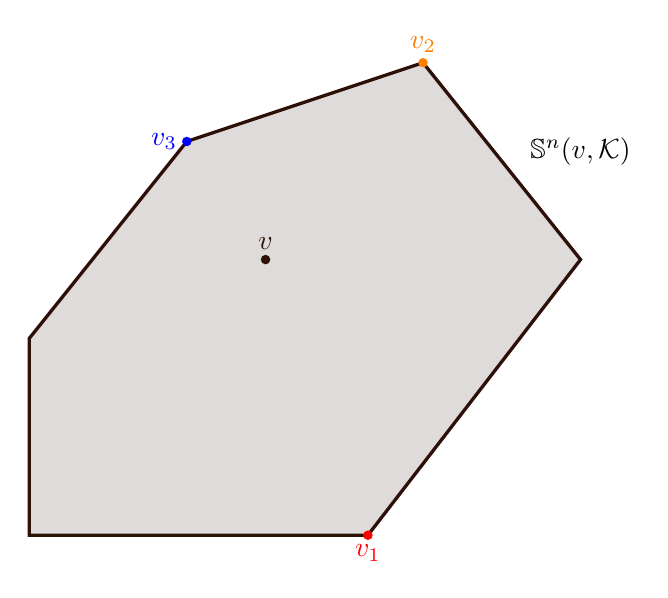
\begin{tikzpicture}[] %%[scale=4] ONLY changes distances, not the canvas
    % Define the coordinates of the vertices
    \coordinate (A) at (0, 0);
    \coordinate (B) at (4.3, 0);
    \coordinate (C) at (7, 3.5);
    \coordinate (D) at (5, 6);
    \coordinate (E) at (2, 5);
    \coordinate (F) at (0, 2.5);
    \coordinate (v) at (3, 3.5);
    \coordinate (v1) at (B);
    \coordinate (v2) at (D);
    \coordinate (v3) at (E);
    
    % Draw and fill the hexagon
		\filldraw[very thick, fill=white!85!mDarkBrown, draw=mDarkBrown] (A) -- (B) -- (C) node[anchor=south,yshift=30]{$\mathbb{S}^n(v,\k)$}-- (D) -- (E) -- (F) -- cycle;

    % \filldraw[mDarkBrown] (A) circle (1pt) node[anchor=north]{$A$};
    % \filldraw[mDarkBrown] (B) circle (1pt) node[anchor=north]{$B$};
    % \filldraw[mDarkBrown] (C) circle (1pt) node[anchor=west]{$C$};
    % \filldraw[mDarkBrown] (D) circle (1pt) node[anchor=south]{$D$};
    % \filldraw[mDarkBrown] (E) circle (1pt) node[anchor=south]{$E$};
    % \filldraw[mDarkBrown] (F) circle (1pt) node[anchor=east]{$F$};

		\filldraw[mDarkBrown] (v) circle (1.5pt) node[anchor=south]{${v}$};
		\onslide<2->{\filldraw[red] (v1) circle (1.5pt) node[anchor=north]{${v_1}$};}
		\onslide<3->{\filldraw[orange] (v2) circle (1.5pt) node[anchor=south]{${v_2}$};}
		\onslide<3->{\filldraw[blue] (v3) circle (1.5pt) node[anchor=east]{${v_3}$};}
		\end{tikzpicture}
	\end{center}
\end{frame}


\begin{frame}{Utopian Gap}
    \begin{itemize}[ ]
        \item<2-> Players are \emph{optimistically biased}.
        \item<3-> As a group made $ v(N) $.
				\item<4-> Players demand $ \red{\shapley[1]{v_1}}, \orange{\shapley[2]{v_2}}, \blue{\shapley[3]{v_3}}, \ldots $
    \end{itemize}
		\vspace{2em}

		\begin{definition}<5->[Utopian Gap]
        The \emph{utopian gap} of $ \left( N, \k, v \right) $ is \[
					\mathcal{G}(v, \k) := \alert<6>{\sum_{i \in N} \shapley[i]{v_i}} - v(N),
        \]
				where $v_i \deq \argmax_{v \in \mathbb{S}(v,\k)} \shapley[i]v$.
			\end{definition}
\end{frame}

\begin{frame}{Reducing $ \mathcal{G} $ -- Setting}
	\begin{itemize}[ ]
		\item<2-> We have \alert<2>{$ v \sim \mathcal{F} $}, where $ \mathcal{F} $ is a distribution of superadditive games.
		\item<3-> We only \alert<3>{know $ \k \supseteq \k_0 $} values of it.
		\item<4-> We have a \alert<4>{budget $ \tau $} of how many values we can learn.
	\end{itemize}
\end{frame}

\begin{frame}{Reducing Optimism Bias -- Offline Approach}
	In the simplest case, we can \alert{minimize the expected value}: \[
		\s^* = \argmin_{\s, \absolute{\s} = \tau} \E_{v \sim \mathcal{F}} \left[ \mathcal{G}(v,\k \cup \s) \right].
	\]

	\vspace{2em}
	We call this the \emph{Offline} approach.
\end{frame}

\begin{frame}{Reducing Optimism Bias -- Online Approach}
	It is \textquote{inefficient} to learn all values at once.

	The \emph{Online} approach seeks to find a policy $ \pi $ which selects the next value to learn based on the values already known.

	A solution to the Online approach can be approximated using reinforcement learning (we use the PPO algorithm).
\end{frame}

\begin{frame}{Reducing Optimism Bias -- Results for $ \mathcal{F} = \texttt{factory} (5) $}
	\begin{center}
		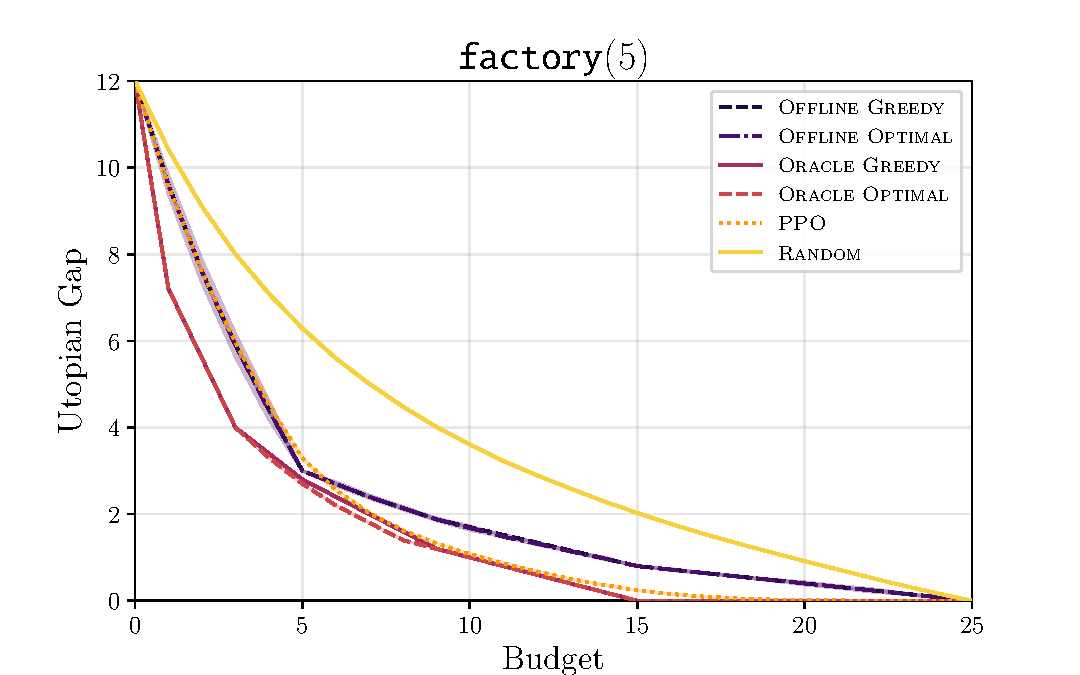
\includegraphics[width=.8\textwidth]{figures/factory5.pdf}
	\end{center}
\end{frame}

\begin{frame}{Reducing Optimism Bias -- Results for $ \mathcal{F} = \texttt{supermodular} (5) $}
	\begin{center}
		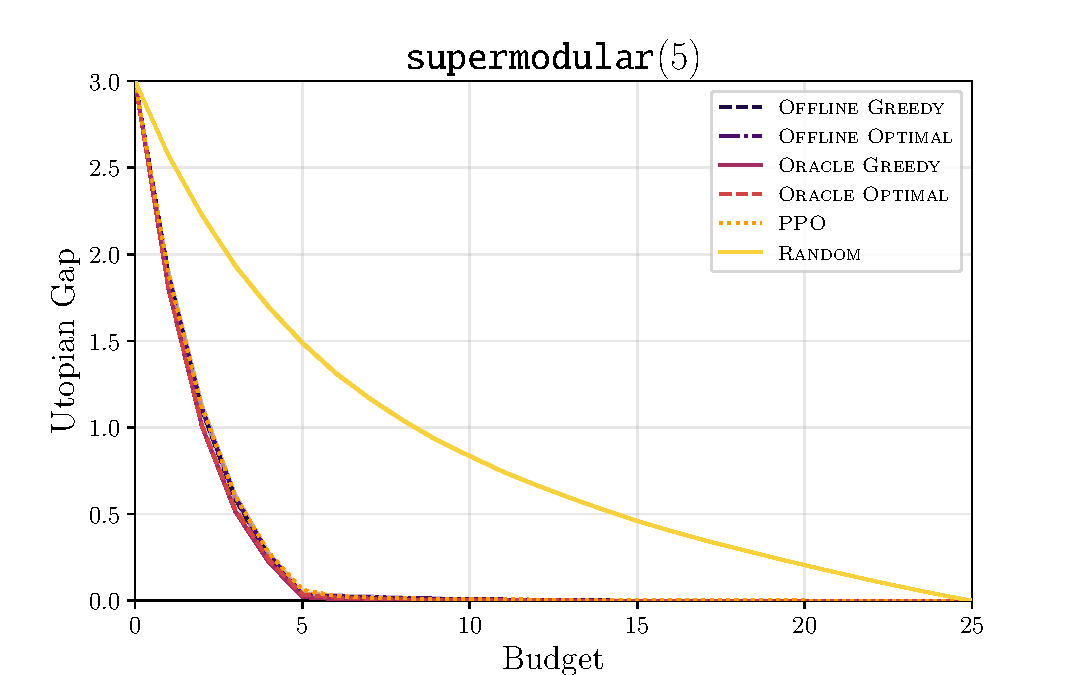
\includegraphics[width=.8\textwidth]{figures/convex5.pdf}
	\end{center}
\end{frame}

\begin{frame}{Reducing Optimism Bias -- \textsc{Largest Coalitions} Heuristic}
	\begin{center}
		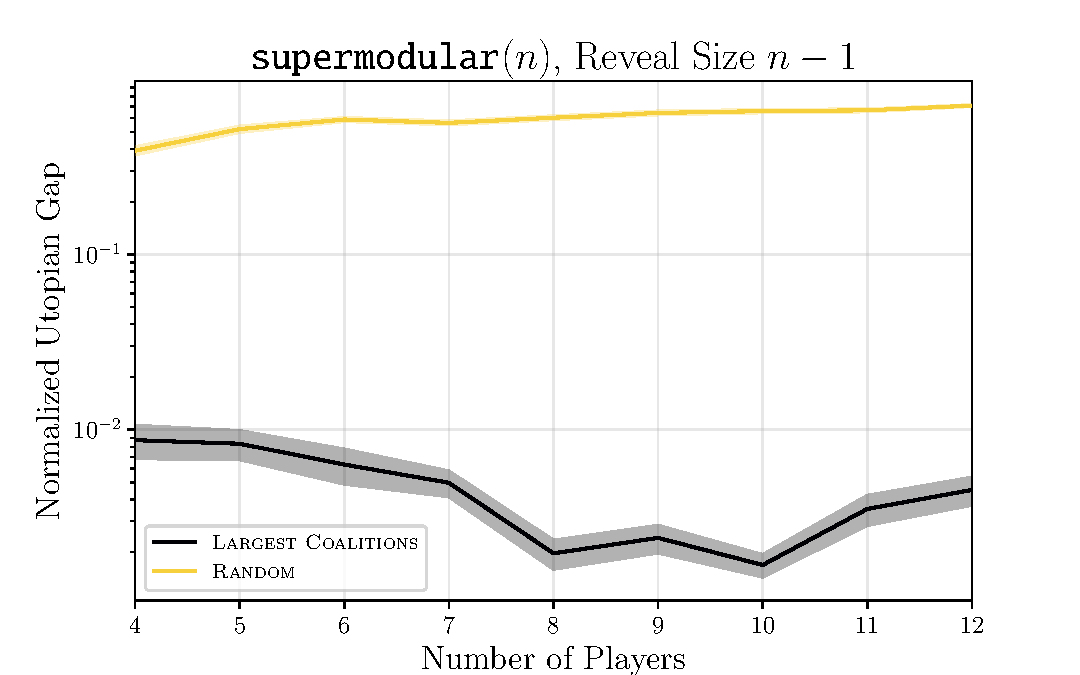
\includegraphics[width=.8\textwidth]{figures/convex_linear.pdf}
	\end{center}
\end{frame}

\section{Thank You!}

\appendix

\begin{frame}{Link}
	\begin{center}
		\qrcode[height=3cm]{https://furadnik.github.io/projects/2024_reducing}

		\vspace{3em}
\texttt{uradnik@kam.mff.cuni.cz}
\\
\texttt{furadnik.github.io}
	\end{center}
	
\end{frame}

\begin{frame}[allowframebreaks]{References}
    \nocite{*}
    \printbibliography[heading=none]
\end{frame}

\end{document}
